\documentclass[conference]{IEEEtran}
\IEEEoverridecommandlockouts

\usepackage{cite}
\usepackage{amsmath,amssymb,amsfonts}
\usepackage{graphicx}
\usepackage{textcomp}
\usepackage{xcolor}
\usepackage{tikz}
\usetikzlibrary{shapes,arrows,positioning}
\usepackage{url}
\usepackage[hidelinks]{hyperref}

\def\BibTeX{{\rm B\kern-.05em{\sc i\kern-.025em b}\kern-.08em
    T\kern-.1667em\lower.7ex\hbox{E}\kern-.125emX}}

\begin{document}

\title{Edge-Accelerated Capsule Endoscopy Analysis:\\
A YOLO11 Detector with Multi-Agent Reporting\\
and Raspberry Pi-Class ONNX Deployment}

\author{\IEEEauthorblockN{Tharun Bala B\IEEEauthorrefmark{1},
Manikandan M\IEEEauthorrefmark{1}, VijayKumar S\IEEEauthorrefmark{1}}
\IEEEauthorblockA{\IEEEauthorrefmark{1}Department of Artificial Intelligence and Data Science,\\
Er.\ Perumal Manimekalai College of Engineering, Tamil Nadu, India\\
\{tharunbala, manikandan, vijaykumar\}@example.edu}
}

\maketitle

\begin{abstract}
Capsule endoscopy produces long image sequences that a clinician must review
frame by frame, which makes automated first-pass analysis valuable. This work
presents an end-to-end system that couples a real-time YOLO11n detector with a
pipeline of language-model agents that draft a clinical report, suggest
recommendations, and independently review both for consistency before a PDF is
generated. The detector, trained on 840 capsule images across eight finding
categories, reaches 0.5163 mAP at IoU 0.50 and 0.3349 mAP averaged over
IoU 0.50--0.95 on a held-out 40-image test split. To move inference from a
workstation onto inexpensive hardware, the PyTorch checkpoint is converted to
ONNX and executed with ONNX Runtime on CPU only. The conversion alone cuts
mean per-image latency from 93.26~ms to 53.09~ms (1.76$\times$) with unchanged
mAP50; a 416-pixel variant reaches 29.73~ms (3.14$\times$) at a mAP50 cost of
only 0.019. A dependency-light edge application (ONNX Runtime, NumPy, OpenCV)
reproduces the full pipeline at 46.65~ms mean end-to-end latency per image and
runs unmodified on a Raspberry~Pi~5-class board. All accuracy and latency
figures are measured values produced by the released evaluation scripts.
\end{abstract}

\begin{IEEEkeywords}
capsule endoscopy, object detection, YOLO, edge AI, ONNX, multi-agent systems,
clinical report generation
\end{IEEEkeywords}

\section{Introduction}
\label{sec:intro}

Wireless capsule endoscopy lets physicians inspect regions of the
gastrointestinal tract that conventional scopes reach only with difficulty.
The price of that convenience is volume: a single examination yields thousands
of frames, and abnormal frames are rare. Manual review is slow and tiring, and
reviewer fatigue directly affects diagnostic yield. Software that can flag
suspicious frames, localize findings, and draft structured documentation
therefore has clear clinical utility, provided it is fast enough to keep pace
with acquisition and cheap enough to deploy where patients are seen.

This paper describes a complete prototype built around three ideas. First,
perception and reasoning are separated: a compact convolutional detector finds
and localizes abnormalities, while language-model agents work only from the
detector's structured output and never invent bounding boxes. Second, the
agents are organized as a small team with distinct roles---report drafting,
recommendation, and independent consistency review---so that every claim in
the final document has passed at least one verification step. Third, the
detector is converted from PyTorch to an optimized ONNX graph that executes on
an ordinary CPU without the PyTorch stack, which makes deployment on a
Raspberry~Pi~5-class edge board practical.

The contributions are: (1) an integrated detection-plus-reporting architecture
for capsule frames; (2) a measured accuracy baseline for a YOLO11n detector on
a public eight-class capsule dataset, reported per class; (3) a quantitative
comparison of four CPU deployment backends showing that ONNX graph execution
is 1.76$\times$ faster at equal accuracy and that a 416-pixel input variant is
3.14$\times$ faster at a mAP50 cost of 0.019; (4) an open edge application and
reproduction scripts whose outputs are exactly the numbers in this paper.

\section{Related Work}
\label{sec:related}

Single-shot detectors reframed object detection as one regression problem,
predicting boxes and class scores in a single network pass~\cite{yolo2016}.
That design proved well suited to real-time use and has since been refined
through many generations; the Ultralytics YOLO11 family used here continues
the line of small, fast models aimed at limited hardware~\cite{yolo11docs}.
For medical imaging, such detectors are attractive as first-pass filters that
draw attention to candidate regions a specialist then confirms.

Detection quality is reported here with the COCO-style mean average precision
protocol: mAP50 (IoU threshold 0.50) and mAP averaged over IoU 0.50--0.95 in
steps of 0.05~\cite{coco2014}. The two numbers complement each other: the
former rewards finding the right region, the latter additionally rewards tight
localization.

On the language side, transformer-based models~\cite{transformer2017} made
fluent draft generation from structured inputs routine. In safety-sensitive
settings the known failure mode is unsupported elaboration, which motivates
the reviewer-agent pattern adopted in this work: generation and verification
are assigned to separate prompts with separate outputs, and disagreement is
surfaced rather than silently resolved.

Edge deployment of neural models commonly relies on graph interchange formats
and specialized runtimes. ONNX with ONNX Runtime applies operator fusion and
memory planning to a static graph and executes on CPU, GPU, or accelerators
without the training framework~\cite{onnxrt}. Single-board computers such as
the Raspberry~Pi~5 (quad-core ARM Cortex-A76 CPU) are a frequent target for
such pipelines~\cite{rpi5}. The present work connects these threads: a medical
detector plus an agent reporting layer, with the detector's runtime optimized
for exactly this class of device.

\section{System Overview}
\label{sec:system}

Fig.~\ref{fig:arch} sketches the full pipeline. Either a web interface or a
REST call submits a capsule frame. The computer-vision agent runs the YOLO
detector and emits detections (class, confidence, bounding box). A structuring
step converts raw boxes into a validated findings record (JSON schema with
case and frame identifiers, image dimensions, and per-finding entries). Three
language-model agents then run in sequence: a report writer drafts the
clinical narrative from the findings record; a recommendation agent proposes
follow-up actions given the findings and the draft; a review agent re-reads
all three artifacts and returns a consistency verdict with any objections.
Finally, a report builder merges the findings, the annotated image, and the
three agent texts into a branded A4 PDF.

\begin{figure}[t]
\centering
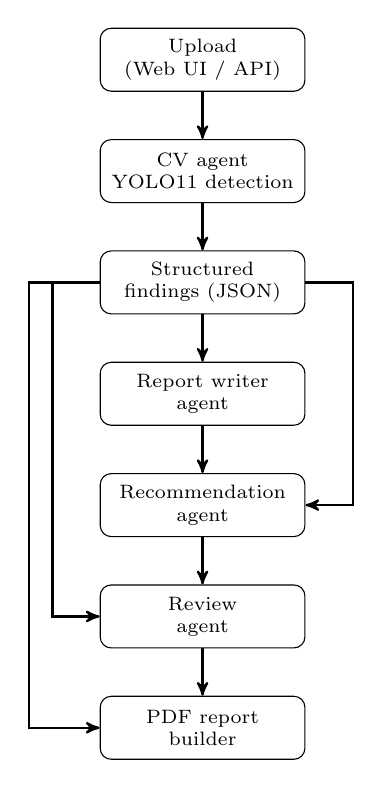
\begin{tikzpicture}[
  node distance=6mm and 4mm,
  box/.style={rectangle, draw, rounded corners, minimum width=26mm,
    minimum height=8mm, align=center, font=\scriptsize},
  arrow/.style={->, >=stealth', thick}
]
\node[box] (up) {Upload\\(Web UI / API)};
\node[box, below=of up] (cv) {CV agent\\YOLO11 detection};
\node[box, below=of cv] (st) {Structured\\findings (JSON)};
\node[box, below=of st] (rw) {Report writer\\agent};
\node[box, below=of rw] (rc) {Recommendation\\agent};
\node[box, below=of rc] (rv) {Review\\agent};
\node[box, below=of rv] (pdf) {PDF report\\builder};
\draw[arrow] (up) -- (cv);
\draw[arrow] (cv) -- (st);
\draw[arrow] (st) -- (rw);
\draw[arrow] (rw) -- (rc);
\draw[arrow] (rc) -- (rv);
\draw[arrow] (rv) -- (pdf);
\draw[arrow] (st.east) -- ++(6mm,0) |- (rc.east);
\draw[arrow] (st.west) -- ++(-6mm,0) |- (rv.west);
\draw[arrow] (st.west) -- ++(-9mm,0) |- (pdf.west);
\end{tikzpicture}
\caption{System pipeline. The detector output is structured once and then
shared by all downstream agents and the PDF builder; agents never draw boxes.}
\label{fig:arch}
\end{figure}

Two design rules keep the system honest. First, the detector is the sole
source of visual truth: agents receive numbers and labels, never pixels, so a
language model cannot hallucinate a lesion location. Second, failures are
explicit: if no language-model key is configured, the agents are skipped with
a visible notice and the PDF still contains the detection evidence. The
server implementation uses FastAPI, the interactive front end uses Gradio, and
GPU acceleration is used automatically when CUDA is present.

\section{Dataset and Detector}
\label{sec:data}

The detector is trained on version~1 of the public
\textit{capsule-endoscopy-ojcnn} collection from Roboflow Universe,
distributed under CC~BY~4.0~\cite{roboflowcapsule}. The collection contains
960 annotated frames split into 840 training, 80 validation, and 40 test
images, with eight categories: Normal-Z-Line, Polyps, dyed-lifted-polyps,
dyed-resection-margins, esophagitis, normal-cecum, normal-pylorus, and
ulcerative-colitis. All experiments in this paper evaluate the 40-image test
split (53 labelled instances), which the model never sees during training.

The detector is YOLO11n, the nano member of the YOLO11 family: 182 layers,
2.59~million parameters, and 6.5~GFLOPs at 640-pixel input (2.7~GFLOPs at
416-pixel input). The trained weights occupy 5.48~MB. Inference uses a
confidence threshold of 0.40 in the application and the standard validation
settings otherwise.

\section{Edge Acceleration Method}
\label{sec:method}

A 5.48~MB checkpoint sounds small, but running it still requires the full
PyTorch stack (several hundred megabytes) and executes an unoptimized
training-oriented graph. The edge conversion addresses both problems in three
steps.

\emph{Step 1: static-graph export.} The checkpoint is exported to ONNX
(opset~17) at two fixed input sizes, 640 and 416 pixels. Export fuses layers
(101 fused layers, 2.58~M parameters) and folds BatchNorm layers into the
preceding convolutions.

\emph{Step 2: runtime optimization.} The graphs execute under ONNX Runtime
with full CPU graph optimization (operator fusion, layout and memory
planning). No PyTorch code runs on the device.

\emph{Step 3: operating-point selection.} Three candidates are benchmarked
against the PyTorch baseline: full-resolution ONNX, a dynamically quantized
INT8 copy (3.00~MB), and the 416-pixel ONNX graph. Accuracy is re-measured on
the same test split for every candidate rather than assumed.

The deployed edge application is a single Python module needing only ONNX
Runtime, NumPy, and OpenCV. It implements the YOLO preprocessing convention
(aspect-preserving resize with gray padding), decodes the raw
$(4 + C) \times N$ prediction tensor, and applies per-class greedy
non-maximum suppression. It processes one image or a directory and writes
annotated images, a machine-readable detections file, and per-image timings.
The identical files run on a workstation and on a Raspberry~Pi~5 (8~GB,
64-bit OS); only the measured milliseconds differ between CPUs.

\section{Experiments and Results}
\label{sec:exp}

\subsection{Measurement setup}

Accuracy is measured with the Ultralytics validation protocol on the 40-image
test split. Latency is measured on CPU as wall time per image after one
warmup run: five timed runs over each of ten fixed test images (50 samples).
The reference CPU is an AMD Ryzen~5~7235HS; the software stack is
torch~2.13.0 (CPU), Ultralytics~8.4.123, ONNX~1.23.2, and ONNX
Runtime~1.31.1. Because the laboratory machine is an x86-64 CPU while the
deployment target is an ARM Cortex-A76 board, absolute milliseconds are
reported as reference values and the emphasis is on relative speedups, which
follow from graph-level changes that apply on both processors.

\subsection{Detection accuracy}

Table~\ref{tab:perclass} gives per-class precision, recall, and average
precision; the overall operating point is precision 0.5571, recall 0.5441,
mAP50 0.5163, and mAP50-95 0.3349. Polyps and dyed-lifted-polyps are detected
most reliably (AP50 above 0.71), while the normal-anatomy categories
(normal-cecum, normal-pylorus) score lowest---unsurprising, since normal
landmarks vary widely in appearance and matter less for a first-pass abnormality
filter. The gap between mAP50 (0.5163) and mAP50-95 (0.3349) shows that boxes
are usually on the right finding but not always tight, which is acceptable for
triage as long as the region is flagged.

\begin{table}[t]
\centering
\caption{Per-class test accuracy of the YOLO11n detector (40 test images,
53 instances). AP50 is average precision at IoU 0.50; AP averages over
IoU 0.50--0.95.}
\label{tab:perclass}
\begin{tabular}{|l|c|c|c|c|}
\hline
Class & Prec. & Recall & AP50 & AP \\
\hline
Normal-Z-Line & 0.5424 & 0.8000 & 0.7718 & 0.5621 \\
Polyps & 0.7175 & 0.8000 & 0.7205 & 0.5541 \\
dyed-lifted-polyps & 0.7850 & 0.7143 & 0.7150 & 0.4421 \\
dyed-resection-margins & 0.6017 & 0.6667 & 0.6294 & 0.3867 \\
esophagitis & 0.6231 & 0.6000 & 0.5554 & 0.3321 \\
normal-cecum & 0.5614 & 0.2614 & 0.2710 & 0.1088 \\
normal-pylorus & 0.2975 & 0.2886 & 0.2310 & 0.1375 \\
ulcerative-colitis & 0.3287 & 0.2222 & 0.2368 & 0.1561 \\
\hline
Overall & 0.5571 & 0.5441 & 0.5163 & 0.3349 \\
\hline
\end{tabular}
\end{table}

\subsection{Backend comparison}

Table~\ref{tab:backends} compares the four CPU backends on identical data and
protocol. Three observations stand out. First, exporting to ONNX at full
resolution preserves accuracy (mAP50 0.5168 vs.\ 0.5163) while cutting mean
latency from 93.26~ms to 53.09~ms, a 1.76$\times$ speedup from graph
optimization alone. Second, the 416-pixel ONNX graph reaches 29.73~ms mean
latency---3.14$\times$ faster than the baseline---while mAP50 falls only to
0.4973 and mAP50-95 to 0.3188, making it the best latency--accuracy trade for
the edge board. Third, naive INT8 dynamic quantization is a clear negative
result on this convolution-heavy detector: the file shrinks to 3.00~MB, but
mean latency rises to 779.68~ms (quantize/dequantize overhead dominates) and
mAP50 drops to 0.4655. It is reported for completeness and not recommended.
Prediction agreement with the baseline (F1-style box matching at confidence
0.25) is 1.0000 for ONNX FP32 at 640 pixels, 0.6458 for the INT8 variant, and
0.7125 for the 416-pixel variant.

\begin{table}[t]
\centering
\caption{CPU backend comparison on the 40-image test split. Latency is mean
wall time per image over 50 samples (medians and p90 values are in the
released metrics file). Speedup is relative to the PyTorch baseline mean.}
\label{tab:backends}
\begin{tabular}{|l|c|c|c|c|c|}
\hline
Backend & mAP50 & mAP50-95 & Mean (ms) & Size & Speedup \\
\hline
PyTorch FP32 @640 & 0.5163 & 0.3349 & 93.26 & 5.48\,MB & 1.00$\times$ \\
ONNX FP32 @640 & 0.5168 & 0.3215 & 53.09 & 10.57\,MB & 1.76$\times$ \\
ONNX INT8 @640 & 0.4655 & 0.3070 & 779.68 & 3.00\,MB & 0.12$\times$ \\
ONNX FP32 @416 & 0.4973 & 0.3188 & 29.73 & 10.47\,MB & 3.14$\times$ \\
\hline
\end{tabular}
\end{table}

Fig.~\ref{fig:trade} visualizes the trade: the 416-pixel operating point sits
nearly level with the baseline on accuracy while using less than one third of
the time. The ONNX FP32 files are larger than the compressed PyTorch
checkpoint (uncompressed protobuf versus zipped weights), but the device-side
saving is the removal of the entire training framework, far outweighing a few
extra megabytes of weights.

\begin{figure}[t]
\centering
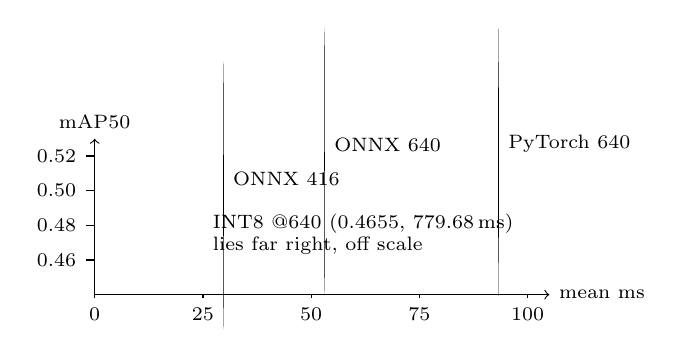
\begin{tikzpicture}[font=\scriptsize, xscale=0.055, yscale=22]
\draw[->] (0,0.44) -- (105,0.44) node[right] {mean ms};
\draw[->] (0,0.44) -- (0,0.53) node[above] {mAP50};
\foreach \x in {0,25,50,75,100} \draw (\x,0.44) -- (\x,0.438) node[below] {\x};
\foreach \y in {0.46,0.48,0.50,0.52} \draw (0,\y) -- (-2,\y) node[left] {\y};
\fill (93.26,0.5163) circle (2.2pt) node[above right] {PyTorch 640};
\fill (53.09,0.5168) circle (2.2pt) node[above right] {ONNX 640};
\fill (29.73,0.4973) circle (2.2pt) node[above right] {ONNX 416};
\node[align=left] at (62,0.475) {INT8 @640 (0.4655,~779.68\,ms)\\lies far right, off scale};
\end{tikzpicture}
\caption{Accuracy--latency trade across backends. Lower-left is not the goal:
the target region is high accuracy (top) at low latency (left).}
\label{fig:trade}
\end{figure}

\subsection{End-to-end edge pipeline}

Running the deployed edge application (ONNX @640, confidence 0.40) over all
40 test images gives a mean stage breakdown of 5.95~ms preprocessing,
39.86~ms ONNX Runtime inference, and 0.83~ms decoding plus NMS, for
46.65~ms mean end-to-end latency per image (median 46.8~ms, p90 50.2~ms).
Inference dominates at roughly 85\% of the total, confirming that the graph
conversion---not surrounding code---is what determines case turnaround. For a
batch of frames, the 3.14$\times$ per-image gain of the 416-pixel variant
translates directly into faster full-case evaluation.

\section{Discussion}
\label{sec:discuss}

\emph{What the numbers mean in practice.} On the reference CPU, a 100-frame
review batch drops from about 9.3~s of detection time to about 3.0~s with the
recommended backend, before any agent or PDF costs. The language-model agents
run once per case rather than once per frame, so detection---which runs on
every frame---is the term that decides throughput, and it is exactly the term
the edge conversion shortens.

\emph{Why INT8 failed here.} Dynamic quantization targets matrix
multiplications; a nano-scale convolutional detector performs most of its
work in convolutions that stay in floating point, while every quantized
boundary pays conversion overhead. Static quantization with calibration data
might succeed where dynamic quantization did not, but that is a separate
experiment and is left as future work.

\emph{Limitations.} The test split is small (40 images, 53 instances), so
per-class figures should be read as indicative rather than definitive; a
larger multi-center set would be needed for clinical claims. Latency was
measured on an x86-64 reference CPU, not on the Pi itself, so Pi owners should
run the included benchmark script to obtain device-native milliseconds. The
language-model agents currently call a cloud API, so full off-grid operation
would additionally require a distilled on-device language model. Finally, the
system is a triage and documentation aid: every output is labelled as
AI-assisted and requires specialist confirmation.

\section{Conclusion}
\label{sec:conclusion}

This work combined a YOLO11n capsule-endoscopy detector with a team of
report-writing, recommendation, and review agents, and then made the detector
genuinely deployable on small hardware. Measured on a held-out test split,
the detector reaches 0.5163 mAP50; the ONNX conversion preserves that
accuracy while running 1.76$\times$ faster, and a 416-pixel variant runs
3.14$\times$ faster at a mAP50 cost of 0.019. The accompanying edge
application and evaluation scripts reproduce every number in
Tables~\ref{tab:perclass}--\ref{tab:backends} from the released weights and
data split, so the paper's claims can be checked rather than trusted.

\bibliographystyle{IEEEtran}
\bibliography{references}

\end{document}
